\section{Sample Memory Distribution} \label{subsec:Sample_Memory_Distribution} 
The ADC converters output are 16 bit sample values and the IS61 external SRAM being used in the project can store 8 bit values, so the 16 bit sample values must be mapped into two 8 bit values in order to be stored in the external memory. The function of the Sample Memory Distribution(SMD) submodule is to split the 16 bit word into two bytes and clock it into, and out of, memory through the read/write module described in section \refq{subsec:Sample_Memory}.

For both read and write operations the SMD module will split the incoming 16 bit sample and address into a \textit{high byte} and \textit{low byte} value and map the values to a 17 bit address. The 8 least significant bits will be stored in the address given to the SMD module from the IV Saver module, the 8 most significant bits will be stored in the same address but with address bit 16 set to 1. This allows for $2^{16} = 65536$ addresses to be used, resulting in $65536\cdot16 \approx \SIQ{1}{\mega\bit}$ of sample storage. This does not use the full capability of the memory chip, but it does fullfill the required sample size. 

The SMD module is build as a finite state machine. This FSM is initialized by the VHDL code seen in listing \ref{lst:7_2_6_FSM_INIT}. Here it can be seen that once a rising edge on "i\_SET" occurs, the "w\_init" signal will be set high. This in turn sets the "w\_RUN" signal to RUN on the next rising edge of the \SIQ{200}{\mega\hertz} master clock. Should "i\_RESET = '1'" or "w\_CMPLT = CMPLT" happen the processes will reset and set "w\_init" to '0' and "w\_RUN" to '0'. This way, when the FSM is complete, it sets "w\_CMPLT" to CMPLT, and the process resets itself. Listing \ref{lst:7_2_6_FSM_INIT} also shows that the HiBYTE, LoBYTE, HiADDR and LoADDR are latched in once the process is initialized. This allows the FSM to use the latched registers during its opperation. 

"LoVal" and "HiVal" in listing \ref{lst:7_2_6_FSM_INIT} are "0b000" and "0b001" respectfully, here as binnary values in c linguistics.

\lstinputlisting[language=C ,style = c,firstnumber=1, linerange=117-140, caption={VHDL code to initialize the FSM for the SMD module.}, label={lst:7_2_6_FSM_INIT}]{Sections/7_SystemDesign/Code/MDIST20.vhd} 

Figure \ref{fig:7_2_6_MemDist} shows a diagram of the Sample Memory Distribution FSM. Here "i\_HOLD" is an input from the Sample Memory module. This is the "o\_ACTIVE" signal, and this allows the FSM to "idle" or "halt" until the Sample Memory module is ready to proceed. In write mode, the FSM works simply by setting the output data to the 8 least significant bits of the input data, and the address to the same address as recieved by the IV Saver. It then sets "o\_SET" high indicating to the Sample Memory module that it should save the current data. It then waits for the Sample Memory module to be ready to recieve data again, and repeats this same action but for the 8 most significant bits at their designated address. The Read opperation works in practically the same manor. Notice that there is no Read/Write control, this is due to the Read/Write setting being controlled by the IV Saver, and this RW signal feeds directly through this module and on to the Sample Memory module.

\begin{figure}[H]
    \centering
    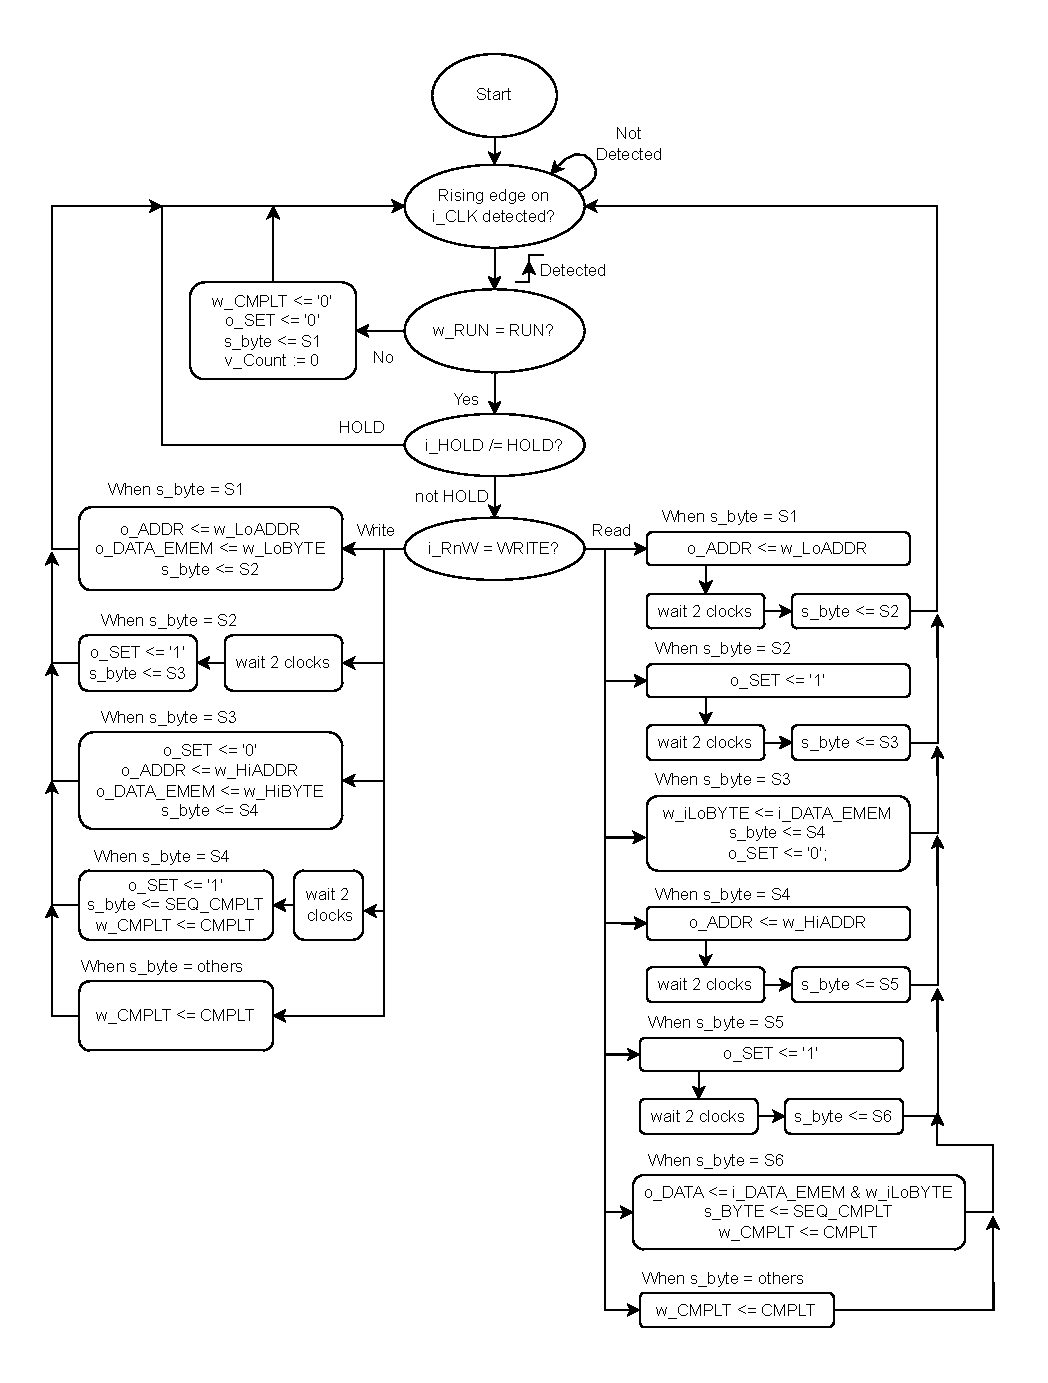
\includegraphics[clip, trim=0 0 0 0, width=1\textwidth]{Sections/7_SystemDesign/Figures/MDIST_FSM.pdf}
    \caption{The module will split an incoming 16 bit word into two bytes and map the address to the 19 bits that the IS61 memory requires.}
    \label{fig:7_2_6_MemDist}
\end{figure}

The SMD module in conjunction with the IV Saver module and Sample Memory module have been tested to reliably save data at a write data-rate of \SIQ{145}{\mega\bit/s}. The SMD module spends roughly \SIQ{80}{\nano\second} to store one 16 bit value. This has been tested by having a busy output for the SMD module. This output consists of the two signals "w\_RUN" and "w\_CMPLT" ored together, this can be seen together with the feedthrough of RW in listing \ref{lst:7_2_6_SMD_BUSY}. The measurements of the output busy flag called "o\_ACTIVE" can be seen appendix in \ref{App:MDIST_BUSY}.

\lstinputlisting[language=C ,style = c,firstnumber=1, linerange=85-87, caption={VHDL code to set RW and output busy flag.}, label={lst:7_2_6_SMD_BUSY}]{Sections/7_SystemDesign/Code/MDIST20.vhd} 